\subsection{Website}

The section describes the website we set up for collecting user preferences.

Figure \ref{fig:website} shows the screenshots of the website.
Figure \ref{fig:website1} is a synthesized screenshot of both \emph{user rating} (top right) and \emph{product recommending} (middle right) user interface. The top left part shows the images of the product. When the user moves the mouse pointer over the image, a larger image will be shown in the top right part, as shown in \ref{fig:website2}. The bottom part of the page shows the textual descriptions of the product.

\begin{figure}[htb]
  \centering
  \subfigure[Synthesized screenshot of both \emph{user rating} and \emph{product recommending} user interface]{
    \label{fig:website1}
    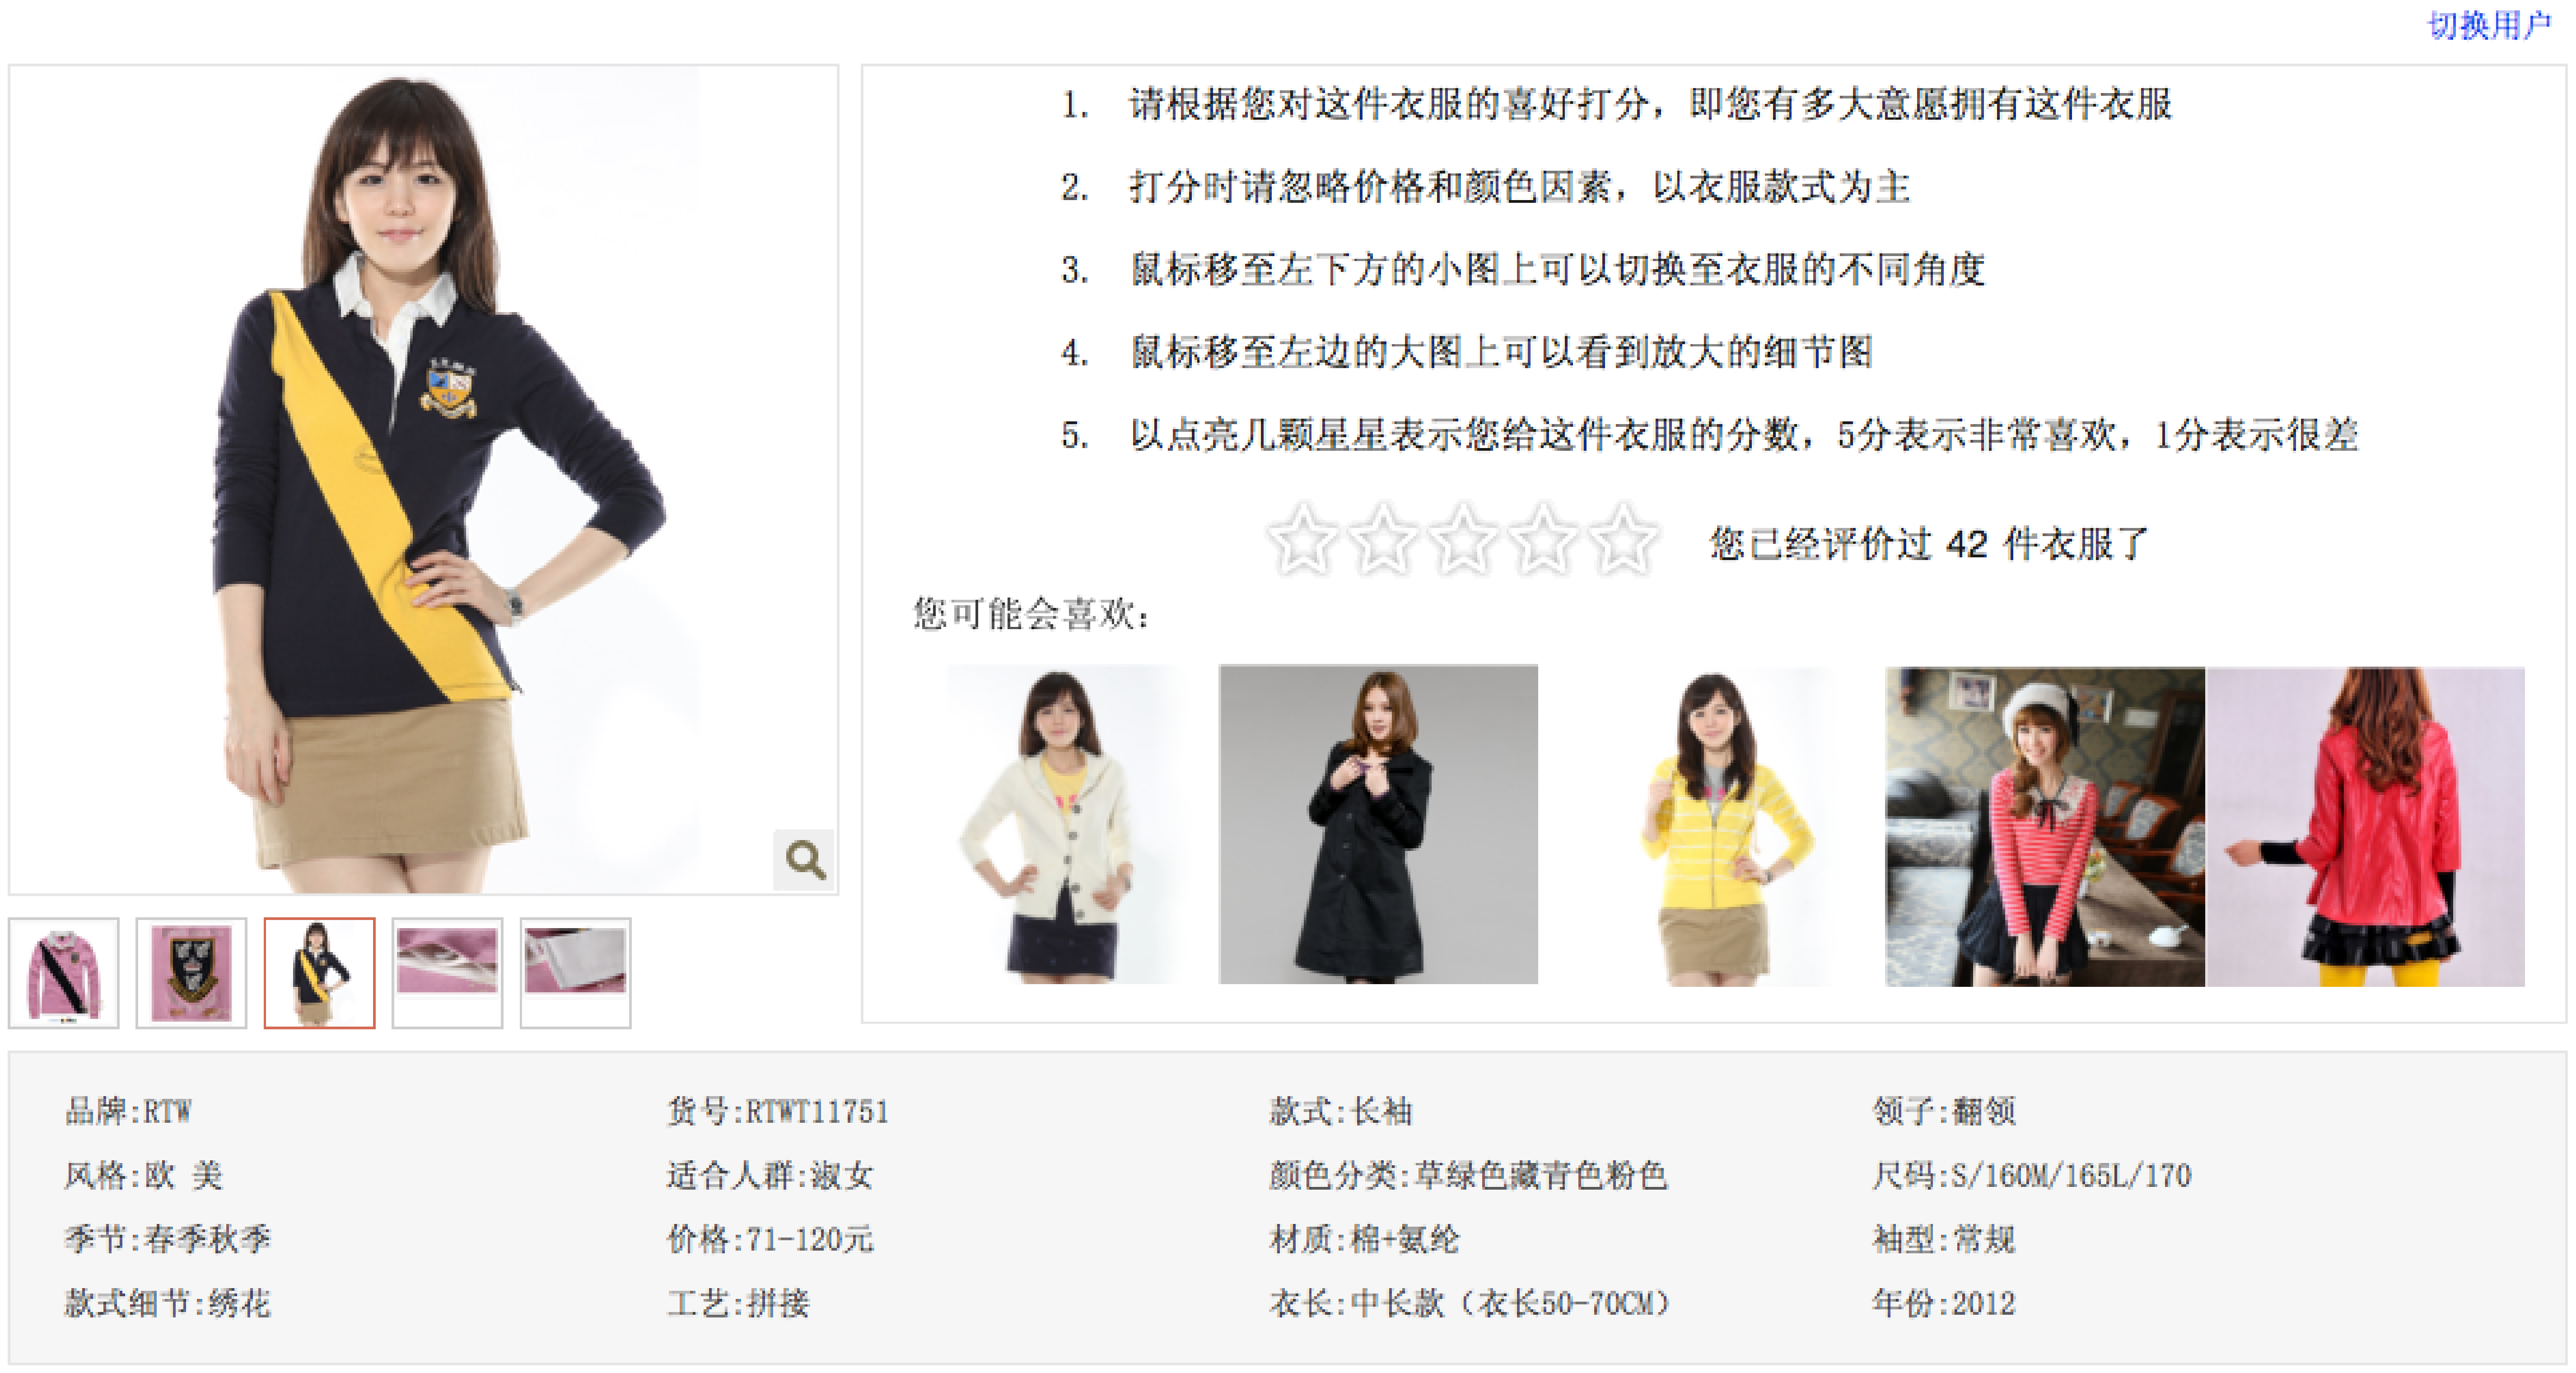
\includegraphics[width=0.8\textwidth]{website1}}
  \qquad
  \subfigure[Screenshot of viewing details of a product image]{
    \label{fig:website2}
    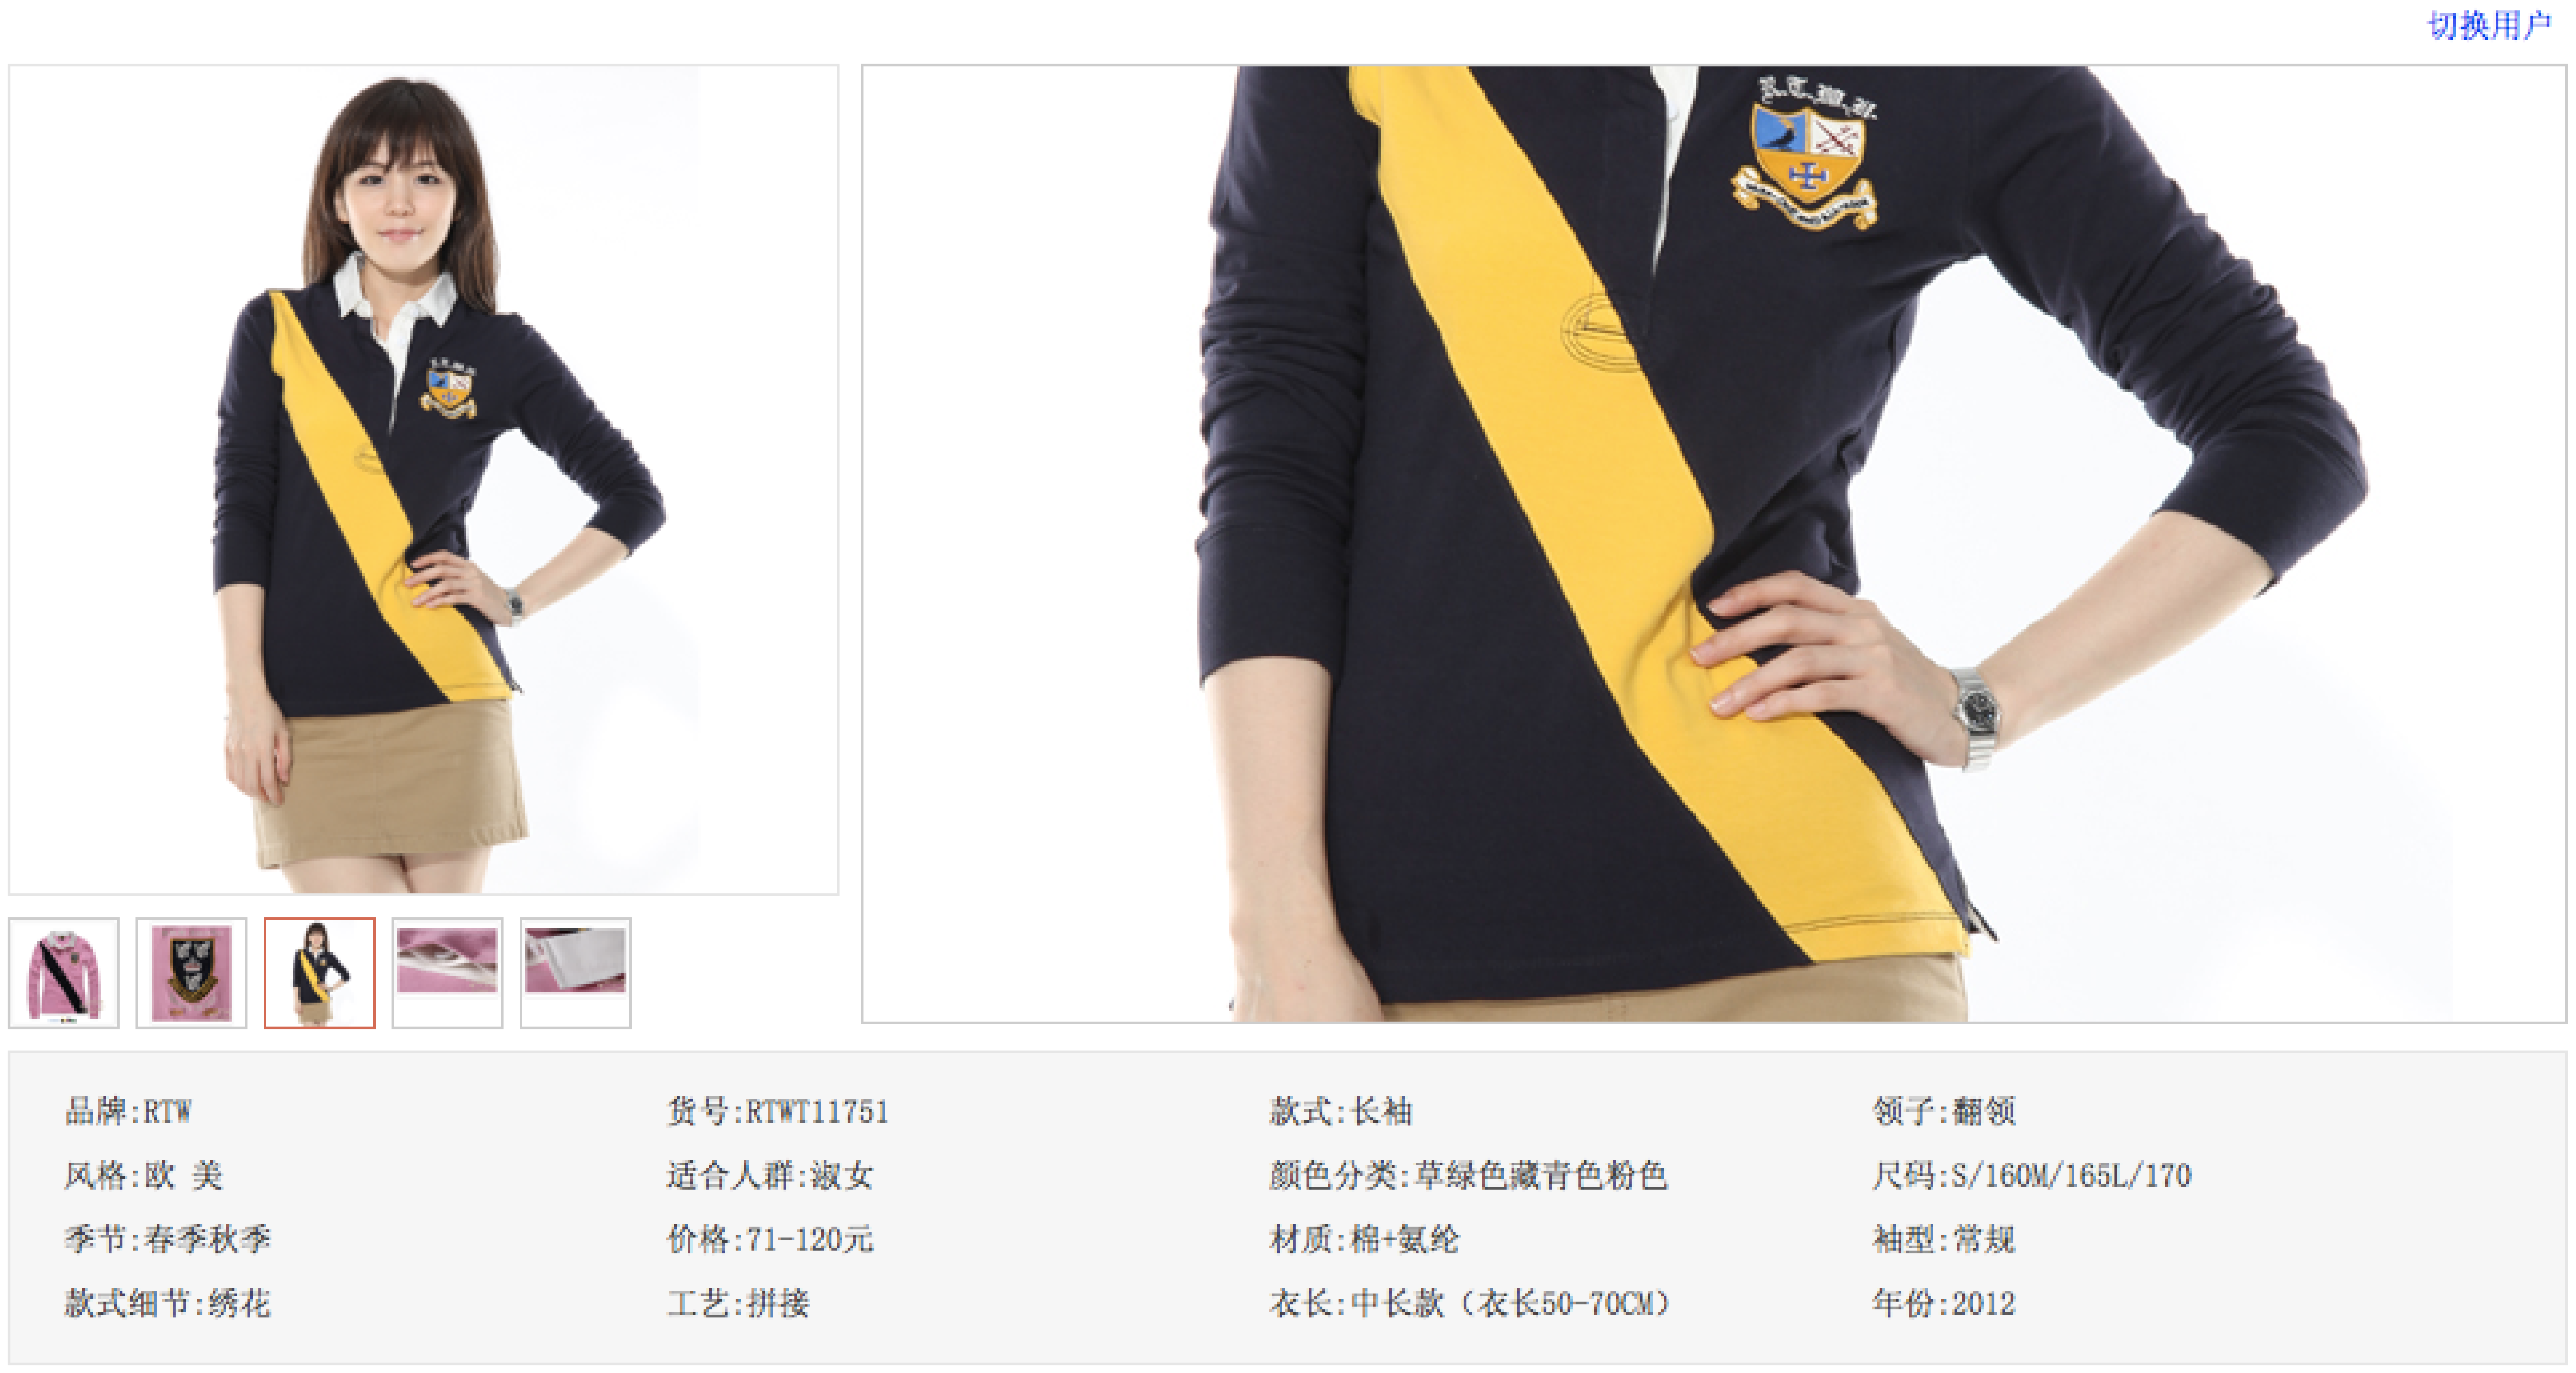
\includegraphics[width=0.8\textwidth]{website2}}
  \caption{Screenshots of our website for collecting user preferences}
  \label{fig:website}
\end{figure}

The website is written in PHP and deployed on Linux with Apache HTTP server. It randomly displays unrated products to the current user, collects user ratings of the products, and stores the ratings to a relational database for further investigation. The source code is available at \url{https://github.com/stfairy/recsys-website}.
